\documentclass[twoside]{article}

\usepackage{lipsum} % Package to generate dummy text throughout this template

\usepackage[sc]{mathpazo} % Use the Palatino font
\usepackage[T1]{fontenc} % Use 8-bit encoding that has 256 glyphs
\linespread{1.05} % Line spacing - Palatino needs more space between lines
\usepackage[utf8]{inputenc}
\usepackage{microtype} % Slightly tweak font spacing for aesthetics

\usepackage[hmarginratio=1:1,top=32mm,columnsep=20pt]{geometry} % Document margins
\usepackage{multicol} % Used for the two-column layout of the document
\usepackage[hang, small,labelfont=bf,up,textfont=it,up]{caption} % Custom captions under/above floats in tables or figures
\usepackage{booktabs} % Horizontal rules in tables
\usepackage{float} % Required for tables and figures in the multi-column environment - they need to be placed in specific locations with the [H] (e.g. \begin{table}[H])
\usepackage{hyperref} % For hyperlinks in the PDF

\usepackage{lettrine} % The lettrine is the first enlarged letter at the beginning of the text
\usepackage{paralist} % Used for the compactitem environment which makes bullet points with less space between them

\usepackage{abstract} % Allows abstract customization
\renewcommand{\abstractnamefont}{\normalfont\bfseries} % Set the "Abstract" text to bold
\renewcommand{\abstracttextfont}{\normalfont\small\itshape} % Set the abstract itself to small italic text

\usepackage{titlesec} % Allows customization of titles
\renewcommand\thesection{\Roman{section}} % Roman numerals for the sections
\renewcommand\thesubsection{\Roman{subsection}} % Roman numerals for subsections
\titleformat{\section}[block]{\large\scshape\centering}{\thesection.}{1em}{} % Change the look of the section titles
\titleformat{\subsection}[block]{\large}{\thesubsection.}{1em}{} % Change the look of the section titles

\usepackage{fancyhdr} % Headers and footers
\pagestyle{fancy} % All pages have headers and footers
\fancyhead{} % Blank out the default header
\fancyfoot{} % Blank out the default footer
\fancyfoot[RO,LE]{\thepage} % Custom footer text

\usepackage{cite}
\usepackage{paralist, tabularx}
\usepackage{graphicx}
\graphicspath{{../images/}}


\usepackage{float}


%----------------------------------------------------------------------------------------
%	TITLE SECTION
%----------------------------------------------------------------------------------------

\title{\vspace{-15mm}\fontsize{24pt}{10pt}\selectfont\textbf{Master thesis proposal}} % Article title

\author{
\large
\textsc{Matthias Jakobs}\\[2mm] % Your name
\normalsize \href{mailto:matthias.jakobs@tu-dortmund.de}{matthias.jakobs@tu-dortmund.de} % Your email address
\vspace{-5mm}
}
\date{}

%----------------------------------------------------------------------------------------

\begin{document}

\maketitle % Insert title

\thispagestyle{fancy} % All pages have headers and footers

%----------------------------------------------------------------------------------------
%	ABSTRACT
%----------------------------------------------------------------------------------------

%\begin{abstract}
\vspace{20px}

%\end{abstract}

%----------------------------------------------------------------------------------------
%	ARTICLE CONTENTS
%----------------------------------------------------------------------------------------

\begin{multicols}{2} % Two-column layout throughout the main article text

\section{Motivation}
\label{sec:motivation}
Human Activity Recognition (HAR) is a task where a signal capturing different human activities (like video) is segmented and classified.
The granularity of the activities to be classified depends on the domain in which HAR is used. 

This master thesis proposes an addition to the works of \cite{reining_towards_2018}, where a framework for HAR in the context of order picking in a warehouse is proposed.
The authors used a motion capturing system in a controlled environment to create a skeleton of the person performing the action.
They propose a pipeline for HAR using \textit{attributes} like \textit{arms reaching forward} and \textit{upper body moving back} as features, extracted from the skeleton data.

A motion capturing system requires strict laboratory conditions.
The goal of this master thesis is to replace the need of motion capturing by utilizing recent advances in 3D human pose estimation from monocular video.
With such a system, a large variety of training data in different, \textit{unconstrained} environments can be captured, hopefully improving the quality of the HAR process.

One advantage of using motion capturing systems to capture human poses is that they do not suffer from occlusion because of the variety of camera angles.
In monocular video, however, occlusion is a serious concern.
For example, the action of holding a phone to ones ear might occlude the hand joint, depending on the camera angle.
Current state-of-the-art methods do not address this problem directly and thus evaluating these models on the occlusion problem and further experimentation in that regard will be the main proposal of this master thesis.

In addition to the direct contribution to \cite{reining_towards_2018}, pose information can be incorporated into HAR for more accurate results \cite{khalid_multi-modal_2018}.
While the authors focused on 2D pose data 3D pose data could improve the accuracy even more. 

%------------------------------------------------
\section{Recent Work}
\label{sec:recent}
3D pose estimation from video developed in recent years, building on the work of 2D pose estimation in still images and video.
The most common approach is to first generate the 2D pose using a dedicated estimator and then \textit{lift} it into the 3D space \cite{pavllo_3d_2019}\cite{martinez_simple_2017}.
This two-step approach outperforms traditional end-to-end approaches \cite{pavllo_3d_2019}.
State-of-the-art 2D pose estimators like \cite{newell_stacked_2016}\cite{wei_convolutional_2016} are often used for generating 2D pose data.
In \cite{wei_convolutional_2016} the authors propose a \textit{pose machine} based on fully convolutional neural networks which refines an initial, local estimation of joint positions through multiple stages.
Each stage increases the receptive field, resolving the ambiguity of local features.
In \cite{newell_stacked_2016} the authors utilize a sequence of \textit{hourglass} modules.
Such a module consists of a symetric architecture where the input gets scaled down through convolution and pooling layers and then scaled back up by nearest neighbor upsampling.
Through skip connections features from previous layers are preserved for use in later layers.

A state-of-the-art model for lifting 2D poses into 3D space was recently proposed by \cite{pavllo_3d_2019}.
One of the key additions is the use of temporal information between single frames.
While some work on video has been done prior (\cite{lin_recurrent_2017}\cite{hossain_exploiting_2018}) the authors approach to temporal information processing achieves state-of-the-art performance on the common benchmarks. 
Also, the authors use different 2D pose estimators based on \cite{he_mask_2017} and \cite{chen_cascaded_2018}.

%Two- and Three stream models for action recognition could be used for just pose estimation

%------------------------------------------------
\section{Method}
% improve pose estimator with regards to occlusion
The main focus of this master thesis will be to tackle the occlusion problem outlined before.
Current 2D pose estimators like \cite{newell_stacked_2016} and \cite{wei_convolutional_2016} will be evalutated on their performance regarding occlusion.
Through experimentation new approaches for tackling occlusion will be proposed.

\begin{figure}[H]
    \centering
    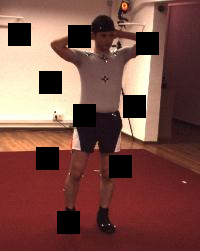
\includegraphics[width=0.4\textwidth]{dropout.png}
    \caption{Example coarse dropout augmentation. The black squares where placed randomly. Because a model needs to fill in the missing information (like a occluded joint) it should become more robust against occlusion. Original image is an example taken from \cite{ionescu_human3.6m:_2014}}
    \label{fig:dropout}
\end{figure}

One experiment will be to train a model using dropout on the training images.
Dropout, in this context, refers to the practice of setting random squares of pixels to pure black while keeping the label unchanged (see \textbf{figure \ref{fig:dropout}}).
Through this procedure, the model may learn to substitute 3D joint locations when occlusion is present in the image.

% end to end training on HAR
Once the pose estimator is robust enough with regards to occlusion a end-to-end training approach for Human Action Recognition is proposed.
% Hier jetzt mehr aus der literatur

%This master thesis proposes to take a subset of the datasets presented in \textbf{section \ref{sec:experiment}.\ref{sec:dataset}} where occlusion happens and evaluate state-of-the-art models on these subsets.
%Through this experimentation, a model will be developed which outperforms the state-of-the-art models on the task of overcoming occlusion while still being competetive on traditional benchmarks.
%Because most of the state-of-the-art models incorporate convolutional neural networks the proposed model will also be based off of these models.


%------------------------------------------------
\section{Experiments}
\label{sec:experiment}
\subsection{Dataset}
\label{sec:dataset}

In evaluating 2D pose estimators, three datasets are most commonly used.
MPII Human Pose \cite{andriluka_2d_2014} is often used for single person and mutli person 2D pose estimation.
Using Youtube videos as source the authors gathered approximately 40,000 annotated images of nearly 500 different actions performed by humans.
These actions include (but are not limited to) activities like skiing, playing music, carrying boxes etc.

In the sport domain, Leeds Sport Pose (LSP) \cite{johnson_clustered_2010} and LSP-Extended \cite{johnson_learning_2011} are often used.
While they focus on a narrow domain many 2D pose estimators were evaluated using these medium sized datasets.

For 3D pose benchmarks, Human3.6M \cite{ionescu_human3.6m:_2014} is widely used.
11 actors perform 17 different scenarios (like eating, talking on phone etc.) in a controlled lab environment wearing motion capturing suits.
The dataset provides 2D and 3D Pose at the same time and is thus widely used for evaluating the lifting task from 2D to 3D described in \textbf{section \ref{sec:recent}}.

In addition to Human3.6M HumanEva I \cite{sigal_humaneva:_2010} is used.
While smaller than Human3.6M, HumanEva I is often used to evaluate specific actions like walking and jogging.

%Maybe: KTH Football II \cite{kazemi_multi-view_2013}

\subsection{Metric}

Most models use the mean per-joint error (in millimeters) as their main metric.
Given the predicted 3D joint locations $x_0^{*}, \dots, x_n^{*}$ for $n$ joints it computes the mean difference given the ground-truth $\hat{x_i}$ using

\newcommand\norm[1]{\left\Vert#1\right\Vert}

\[
    e = \frac{1}{n} \sum_{i=1}^{n} \norm{\hat{x_i} - x_i^{*}}_2
\]

As this metric does not take different scales and orientation into account, the root locations of the vectors are aligned to make the results translation invariant and better comparable.

%\textbf{single person, single image:} Percentage of Correct Keypoints (PCK), PCKh, Percent of Detected Joints (\cite{toshev_deeppose:_2014})


%------------------------------------------------
%   REFERENCE LIST
%------------------------------------------------
\bibliographystyle{acm}
\bibliography{../bibliography}
%----------------------------------------------------------------------------------------

\end{multicols}

\end{document}
